\documentclass[border=10pt]{standalone}
\usepackage{tikz}
\usepackage{amsmath,amssymb}
\usetikzlibrary{decorations.markings,arrows.meta}

\begin{document}
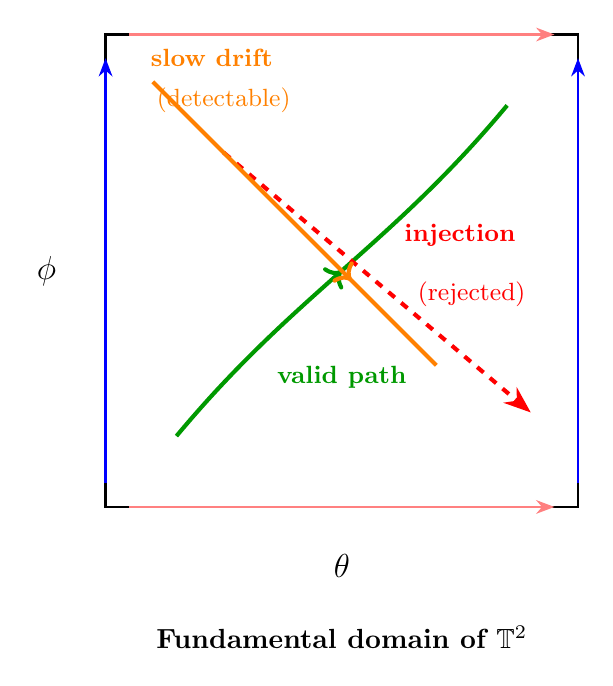
\begin{tikzpicture}[scale=3]
    % Draw torus representation as a square with identified edges
    \draw[thick] (0,0) rectangle (2,2);

    % Arrows indicating identification
    \draw[-{Stealth},thick,blue] (0,0.1) -- (0,1.9);
    \draw[-{Stealth},thick,blue] (2,0.1) -- (2,1.9);
    \draw[-{Stealth},thick,red!50] (0.1,0) -- (1.9,0);
    \draw[-{Stealth},thick,red!50] (0.1,2) -- (1.9,2);

    % Normal trajectory (smooth curve) - VALID PATH
    \draw[thick,green!60!black,line width=1.5pt,decoration={markings,mark=at position 0.5 with {\arrow{>}}},postaction={decorate}]
        (0.3,0.3) .. controls (0.8,0.9) and (1.2,1.1) .. (1.7,1.7);
    \node[green!60!black,font=\small\bfseries] at (1.0,0.55) {valid path};

    % Injection attempt (sharp jump) - shown as dashed - REJECTED
    \draw[thick,red,dashed,line width=1.5pt,-{Stealth}] (0.5,1.5) -- (1.8,0.4);
    \node[red,font=\small\bfseries] at (1.5,1.15) {injection};
    \node[red,font=\small] at (1.55,0.9) {(rejected)};

    % Slow drift attack - DETECTABLE
    \draw[thick,orange,line width=1.5pt,decoration={markings,mark=at position 0.7 with {\arrow{>}}},postaction={decorate}]
        (0.2,1.8) .. controls (0.4,1.6) and (0.6,1.4) .. (0.8,1.2)
        .. controls (1.0,1.0) and (1.2,0.8) .. (1.4,0.6);
    \node[orange,font=\small\bfseries] at (0.45,1.9) {slow drift};
    \node[orange,font=\small] at (0.5,1.72) {(detectable)};

    % Labels
    \node[font=\large] at (1,-0.25) {$\theta$};
    \node[font=\large] at (-0.25,1) {$\phi$};

    % Title
    \node[font=\bfseries] at (1,-0.55) {Fundamental domain of $\mathbb{T}^2$};
\end{tikzpicture}
\end{document}
